\newpage
\subsection{Activities} \index{Activity}
\label{sec:Activities}
Die Warranty App besteht aus drei verschiedenen Activities mit unterschiedlichen Aufgaben.
\\
Die \textit{CardListActivity} ist die eigentliche Haupt- Activity und dient als Einstieg in die App. Diese Activity stellt je eine Funktion zur Bearbeitung bereits existierender Quittungen sowie eine Funktion zur Erstellung eines neuen Eintrags bereit.
\\
Beim Ausw�hlen der Bearbeitungs- Funktion wird der Benutzer in die \textit{CardActivity} geleitet, die es ihm erm�glicht s�mtliche Details eines Eintrages zu bearbeiten. Mit der Speichern- Funktion wird der Eintrag in der Datenbank aktualisiert und der Benutzer zur�ck zur \textit{CardListActivity} geleitet.
\\
Die aufgenommen Bilder werden von der \textit{CardActivity} aus mit Hilfe der von Android bereitgestellten Gallery App dargestellt.
\\
Durch die Auswahl der Erstellungs- Funktion gelangt der Benutzer direkt die \textit{PhotoActivity}, die nebst weitern Funktionen die von Android bereitgestellte Kameraapplikation aufruft. Nach der Aufnahme eines Fotos wird ohne User- Interaktion in die oben erw�hnte \textit{CardActivity} gewechselt.
\\

\begin{figure}[h!]
	\label{fig:Warranty_Flowchart}
	\centering
	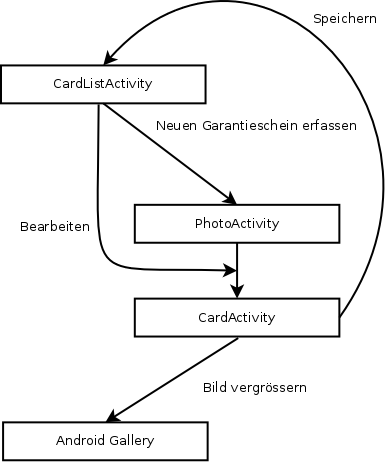
\includegraphics[width=0.5\textwidth]{Flowchart_Warranty.png} 
	\caption{Flowchart Warranty}
\end{figure}